% CONSIDERAÇÕES FINAIS--------------------------------------------------------------------

\chapter{Considerações Finais}
\label{chap:consideracoesFinais}

% TODO: ajustar a conclusão, incluir futuras versões, relatar mais claramente sua função e o qual foi a importância para o projeto.

O sistema passou a ser utilizado em sua plenitude a partir de agosto de 2017 e em 2018 terminou o ano sendo o 4º sistema mais usado em todo o TRE com 23.375 transações conforme \autoref{fig:figura-ranking2018}. Já em 2019, até março foram registradas 4.006 transações já sendo o 3º sistema mais utilizado.

\begin{figure}[!htb]
    \centering
    \caption{Veículos - Ranking 2018}
    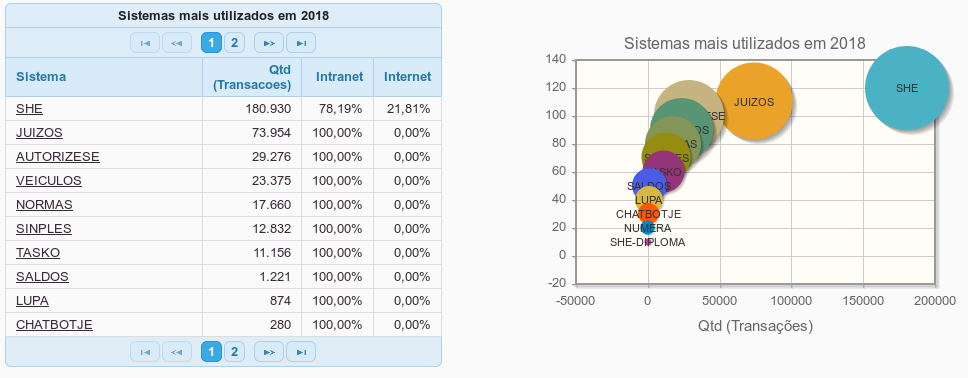
\includegraphics[width=0.75\textwidth]{./dados/figuras/ranking2018.png}
    \fonte{SEDES}
    \label{fig:figura-ranking2018}
\end{figure}

A experiência de estágio no TRE-PB adicionou propriedade aos conhecimentos adquiridos ao longo da minha jornada como aluno e desenvolvedor de sistemas para internet. 
Durante os dois anos de estágio fui incluído em uma rotina de trabalho equivalente as teorias e práticas vistas e desenvolvidas em sala de aula. 
Fui amparado por excelentes profissionais, sempre dispostos a dar o seu melhor tanto para o ambiente de trabalho quanto para uma sociedade melhor e mais justa.

Assistir uma boa aula, realizar os exercícios em sala e ainda repetir todo esse processo durante o estágio proporcionou, sem dúvidas, um crescimento imensurável ao meu intelecto. Tive a oportunidade de participar de alguns projetos, dentre eles o \imprimirtitulo \space, o qual participei já na primeira reunião até seu encerramento. Poder opinar, dar sugestões, incluir classes inteiras ao projeto, compilar o código e realizar o deploy da aplicação, até mesmo em produção me fez acreditar que eu estava no caminho correto e que seria possível me apresentar diante de qualquer empresa como um verdadeiro profissional.

Durante o projeto me deparei com situações de grande dificuldade, as vezes por não conseguir codificar a solução do problema, outras pelo tamanho da responsabilidade envolvida. Sempre fui encorajado a encontrar a solução, investigar, às vezes por dias.
Fiz parte de uma equipe sempre pronta e disposta a resolver suas demandas de trabalho, esclarecer dúvidas, sempre discutindo possibilidades de melhorar. Sinto orgulho em dizer que, durante meu estágio, todos os desenvolvedores efetivos do TRE-PB foram alunos IFPB.

Saio satisfeito dessa jornada, sabendo que pude absorver o máximo do que foi exposto durante o curso e o estágio. Tratando-se de tecnologias, muito ainda é pouco. Tudo que aprendi e vivi serve apenas como base para minha carreira como desenvolvedor. Conquistei apenas a ponta do iceberg, tenho plena clareza que falta muito a aprender e evoluir ainda. 